\begin{tikzpicture}[scale=1/2]

%    \def\lenreg{2};
%    \def\diam{3};
    \def\spy{2};
    \def\xdist{8cm};
    \def\ydist{-7cm};
%    \def\persp{20};
%    
%    \def\LX{1};
%    \def\LY{2};
%    \def\CoreX{1.5};
%    \def\CoreY{.9*\LY};
%    

	\def\L{2.1};
	\def\R{5};
	\def\HX{.25};
	\def\decalage{\R/2-\L/2};
	
%	\draw[opacity=0] (\decalage,0) rectangle ++(-\HX,\R); %%% Pour l'alignement vertical
	
	\begin{scope}[xslant=1,yscale=.5]
		\draw(6.5,\R/2) node{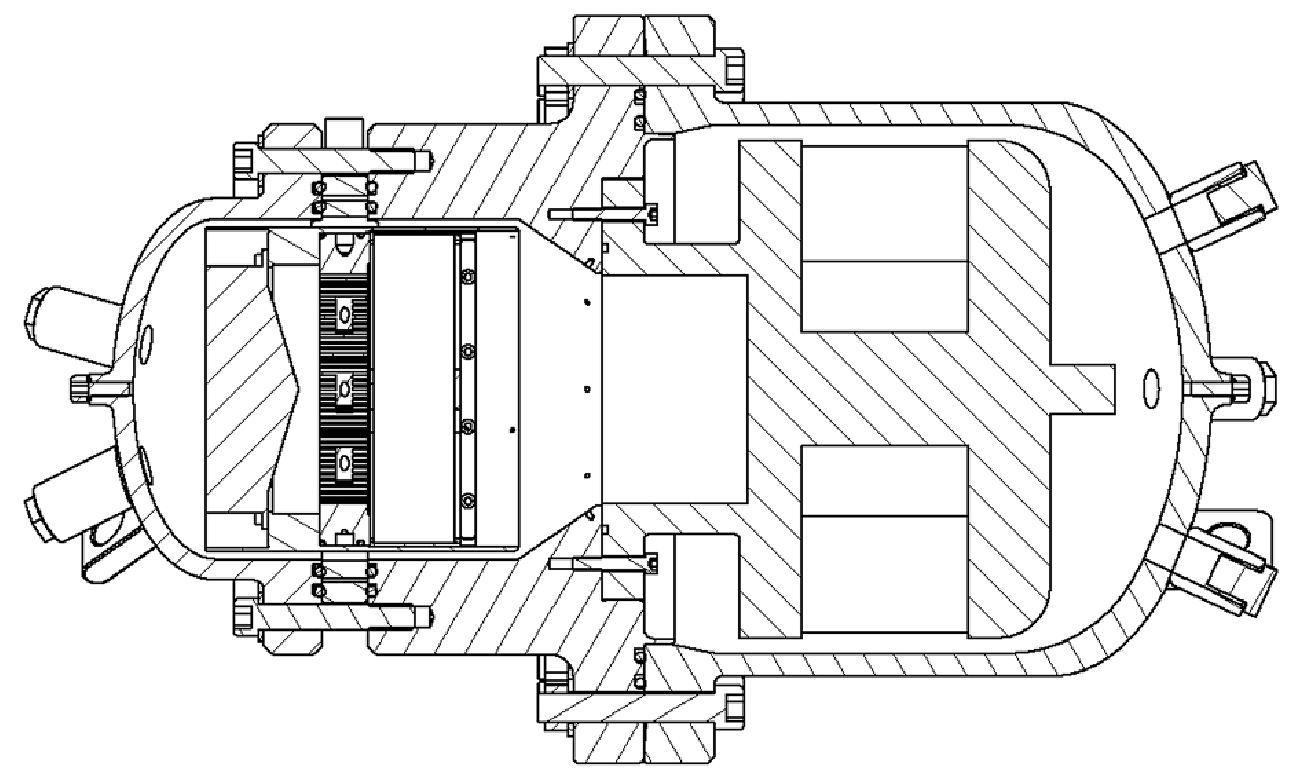
\includegraphics[width=.9\textwidth]{../fig/fig_OrientationCore/tex/TACOT.png}};	
	
		\fill[shading=axis,right color=MatlabBlue,left color=MatlabOrange, shading angle=45, draw=black] (\decalage,0) rectangle ++(\L,\R);
		\draw[fill=MatlabOrange] (\decalage,0) rectangle ++(-\HX,\R);
		\draw[fill=MatlabBlue] (\decalage+\L,0) rectangle ++(\HX,\R);

		\foreach \z [evaluate=\z] in {0,...,4}{
			\foreach \r [evaluate=\r as \num using int(\r+1 + 3*\z)] in {0,...,2}{
				\draw ({\decalage+.5+\L-\z*(1+\L)/4},{-(\R-.4)/2*\r+\R-.2}) node[minimum size=10pt,draw,circle,fill=white,opacity=.7,text opacity=1]{} node(n\z\r){\scriptsize \num};
}}

%		\draw (n01.east) node [right]{$\rightarrow$ \begin{tabular}{l}Source\\acoustique\\principale\end{tabular}};
		\draw ($(n01)+(1.5,0)$) node[minimum size=10pt,draw,circle,fill=white,opacity=.7,text opacity=1]{} node {\scriptsize 0};% node[anchor=west]{\begin{tabular}{rl}
%		& Src\\
%		$\rightarrow$ & ac\\
%		& princ
%		\end{tabular}};
		\draw (n30.north west) node [above, fill=white, fill opacity=.7, text opacity=1]{\textcolor{MatlabOrange}{\textbf{Ambiant}}};
		\draw (n10.north east) node [above, fill=white, fill opacity=.7, text opacity=1]{\textcolor{MatlabBlue}{\textbf{Froid}}};
	\end{scope}
	
	
		
\end{tikzpicture}